%---------------------
% START OF PREAMBLE - do not delete!
%---------------------
\documentclass[12pt]{article}
\usepackage[pdftex]{graphicx}
\usepackage{amsmath}
\usepackage{verbatim}
\DeclareGraphicsRule{*}{mps}{*}{}

%==============================================================================
% Page layout
%==============================================================================

%------------------------------------------------------------------------------
%  Define the page dimensions.
%------------------------------------------------------------------------------
\setlength{\hoffset}{0.0in}
\setlength{\oddsidemargin}{0.0in}
\setlength{\evensidemargin}{0.0in}
\setlength{\textwidth}{6.75in}

\setlength{\voffset}{0in}
\setlength{\topmargin}{-.6in}
\setlength{\headheight}{12pt}
\setlength{\headsep}{12pt}
\setlength{\textheight}{9.5in}
\renewcommand{\baselinestretch}{1.0}
\renewcommand{\labelitemi}{-}

% writing the section number and the subsection number together
% and also the subsubsection in the form of 1.a
\renewcommand\thesubsection{\arabic{section}.\alph{subsection}}
\renewcommand\thesection{Problem \arabic{section}}
%------------------------------------------------------------------------------

%---------------------
% END OF PREAMBLE - do not delete!
%---------------------
\begin{document}

%---------------------
% make the title
%---------------------
\begin{titlepage}
\centering
{\LARGE\bfseries Homework 2}

\vspace{1cm}

{\Large Aerosol Physics, Chemistry, Clouds and Climate}

\vspace{2cm}

{\large Masoud Akbarzadeh}

\vspace{2cm}

{ \today }

\vfill

{\itshape Colorado State University}
\end{titlepage}


%---------------------

%---------------------
% begin main text
%---------------------
\section{Condensation}\label{sec:problem-1}
\subsection{}\label{subsec:problem-1-a}
Assumed values:
\begin{itemize}
    \item $T = 298.15K$
    \item $P = 1atm$
    \item $C_\infty = 5E7\ molecules\ cm^{-3} = 8.14E(-12)\  kg\ m^{-3}$
    \item $C_s = 0$
    \item $D_g = 1E(-5)\ m^2\ s^{-1}$
    \item Equation used for the condensation diameter growth rate:
\end{itemize}

\[\frac{dD_p}{dt}=\frac{4D_g}{\rho D_p}(C_\infty-C_s)\beta\]

\begin{figure}[H]\label{fig:problem-1-a}
    \begin{center}
        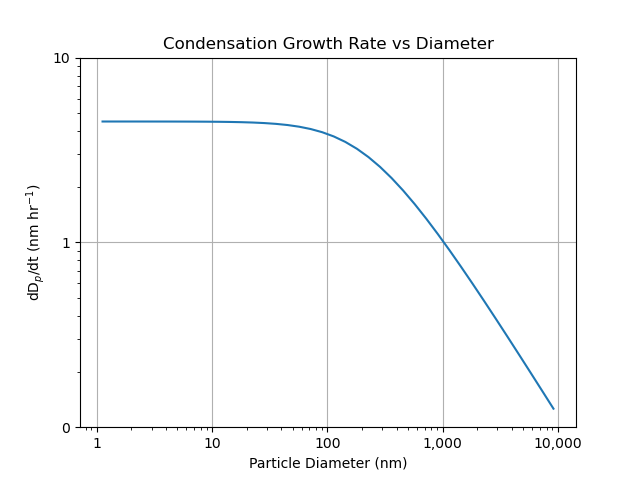
\includegraphics[width=5in]{hw2_pr1_1_condensation_growth_rate_vs_diameter.png}
        \caption{Problem(1) part(a) Condensation diameter growth rate vs diameter}
    \end{center}
\end{figure}

The figure ~\ref{fig:problem-1-a} shows the condensation diameter growth rate vs diameter.
The condensation growth rate is independent of the diameter of the particle in the kinetic regime($D_p < 10nm$).
Whereas in the continuum regime($D_p > 1000nm$), the condensation diameter growth rate is inversely proportional to the diameter of the particle.
In the transition regime($10nm < D_p < 1000nm$), the condensation diameter growth rate is a function of the diameter of the particle and behaves similar to a sigmoid function between the kinetic and continuum regimes.



\subsection{}\label{subsec:problem-1-b}

 In order to calculate condensation mass growth rate the following equation was used:
\[\frac{dM_P}{dt}=J=2\pi D_g D_p(C_\infty-C_s)\beta\]


\begin{figure}\label{fig:problem-1-b-2}
    \begin{center}
        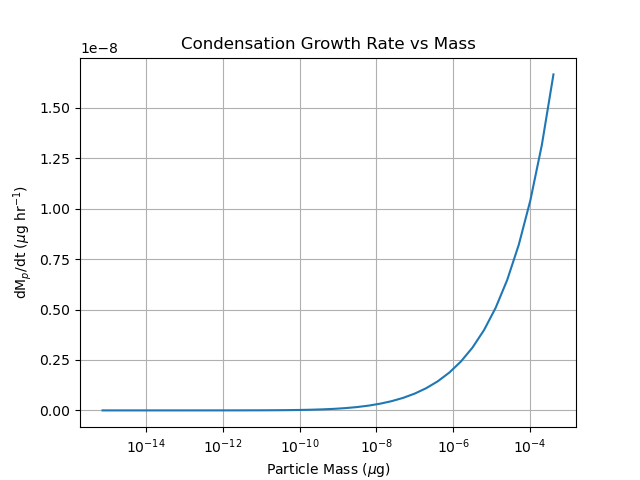
\includegraphics[width=5in]{hw2_pr1_2_condensation_growth_rate_vs_mass.png}
        \caption{Problem(1) part(b) Condensation mass growth rate vs particle diameter}
    \end{center}
\end{figure}




%new page
\newpage
\section{Coagulation}\label{sec:problem-2}
% part A of problem 2 % subsection written in form of 2.a
\subsection{Coagulation kernel and rate}\label{subsec:problem-2-a}
Assumed values:
\begin{itemize}
    \item $T = 298.15K$
    \item $P = 1atm$
    \item $N_1 = 3000\ cm^{-3},\ D_p1 = 10nm $
    \item $N_2 = 400\ cm^{-3},\ D_p2 = 100nm $
    \item $D_g = 1E(-5)\ m^2\ s^{-1}$
\end{itemize}
Fuchs form of the brownian coagulation ceofficient K_{12}: \\ \\
\\
$\displaystyle K_{12} = 2\pi(D_1+D_2)(D_{p1}+D_{p2})(\frac{D_{p1}+D_{p2}}{D_{p1}+D_{p2}+2(g_1^2+g_2^2)^{1/2}}+\frac{8(D_1+D_2)}{(c_1^2+c_2^2)^{1/2}(D_{p1}+D_{p2})})^{-1}$
\\ \\
$\displaystyle K_{12} = 2.38E(-8)\  cm^3 s^{-1}
\\ \\
K_{table13.3}=2.5E(-8)\ cm^3 s^{-1}$
\\ \\
$J_{12} = K_{12}N_1N_2 = 2.85E(-2)\ cm^{-3} s^{-1}$

\subsection{Frequency of collision}\label{subsec:problem-2-b}
The frequency of collision with the smaller particles$=K_{12}N1=7.13E(-5)$
\\\\
The frequency of collision =  $\displaystyle\frac{Collision\ rate}{N_1}$

\subsection{Growth rate due to coagulation}\label{subsec:problem-2-c}
The growth rate due to coagulation is given by the following equation:
\\ \\
$\displaystyle \frac{dV_p_2}{dt}=k_{12} N_1 V_p_1 $
\\ \\
$\displaystyle \frac{dD_p_2}{dt}=k_{12} N_1 V_p_1 \frac{2}{\pi D_p_2^2}$
\\ \\
$\displaystyle \frac{dD_p_2}{dt}= 8.56E(-3) nm\ hr^{-1}$

\subsection{Growth in 1 week}\label{subsec:problem-2-d}
The percent change in diameter in 1 week = 1.44\%
\\
The percent change in mass in 1 week = 4.31\%
\newpage

\begin{figure}\label{fig:problem-2-a-1}
\begin{center}
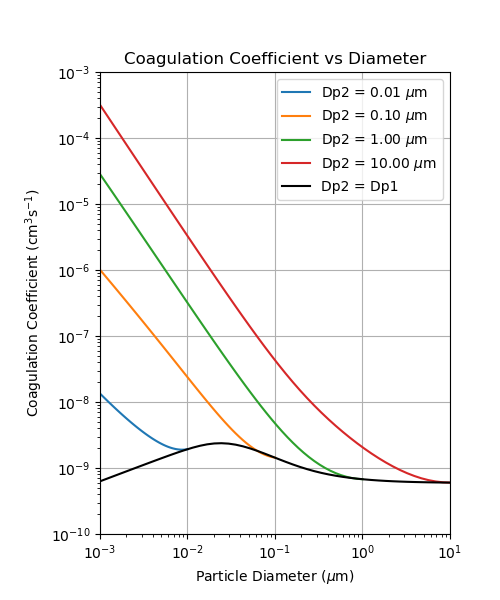
\includegraphics[width=3in]{hw2_pr2_1_coagulation_coefficient_vs_diameter}
\caption{Fuchs Coagulation the code}
\end{center}
\end{figure}

\begin{figure}\label{fig:problem-2-a-2}
\begin{center}
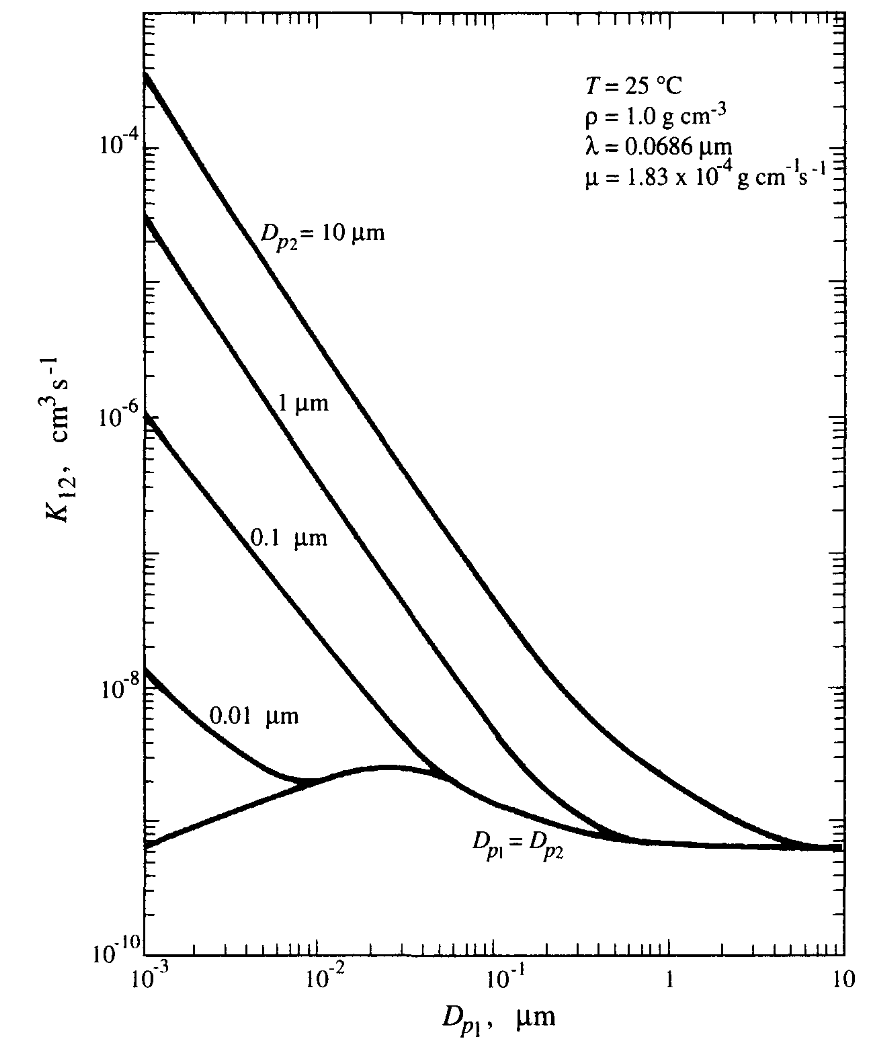
\includegraphics[width=3in]{Table_13_5_Fuchs_Coagulation_plot.png}
\caption{Table\_13\_5 Fuchs Coagulation plot}
\end{center}
\end{figure}



\end{document}


